
\documentclass{beamer}
% logo of my university
\titlegraphic{
\includegraphics[width=4cm]{images/rust}%
}
\author{Roel Deckers}
\institute{Uppsala University}
\begin{document}
  %key points:
  %   performance, almost-zero(tm) overhead
  %   safety (openSSL), no null pointer, no dangling pointers, no buffer overruns
  %   Compile-time, no garbage collector
  %   compatible
  %   Cargo
  %   Great and growing community. Not an easy language, but easy to get started.
  %   Quotes from people.

\begin{document}
\begin{frame}
\titlepage
\end{frame}

  \begin{frame}
    \frametitle{Rust...?}
    \begin{itemize}
      \item{systems-programming language:} like C.
      \item{It's completely memory safe:} at compile time, no GC needed.
      \item{First class multithreading support}.
      \item{Blazingly fast}.
    \end{itemize}
  \end{frame}

  \begin{frame}
    \frametitle{Bugs, what bugs?}
    \begin{itemize}
      \item{Heartbleed!} 
\includegraphics[height=2cm]{images/heartbleed}
      \item{Stagefright!} 
\includegraphics[height=1.5cm]{images/stagefright}
      \item{Shellshock..?} 
\includegraphics[height=2cm]{images/Shellshock-bug}
    \end{itemize}
  \end{frame}

\begin{frame}
  \frametitle{So, what can you make with Rust?}
\begin{figure}

\includegraphics[width=0.9\textwidth]{images/servo}
\caption{a webbrowser}
\end{figure}
\end{frame}

\begin{frame}
  \frametitle{So, what can you make with Rust?}
\begin{figure}
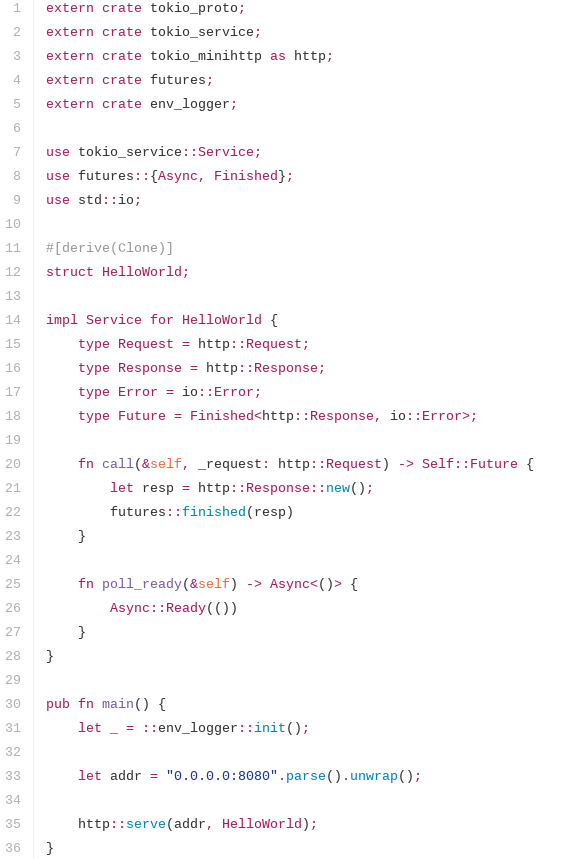
\includegraphics[width=0.4\textwidth]{images/tokio}
\caption{a webserver}
\end{figure}
\end{frame}

\begin{frame}
  \frametitle{So, what can you make with Rust?}
\begin{figure}
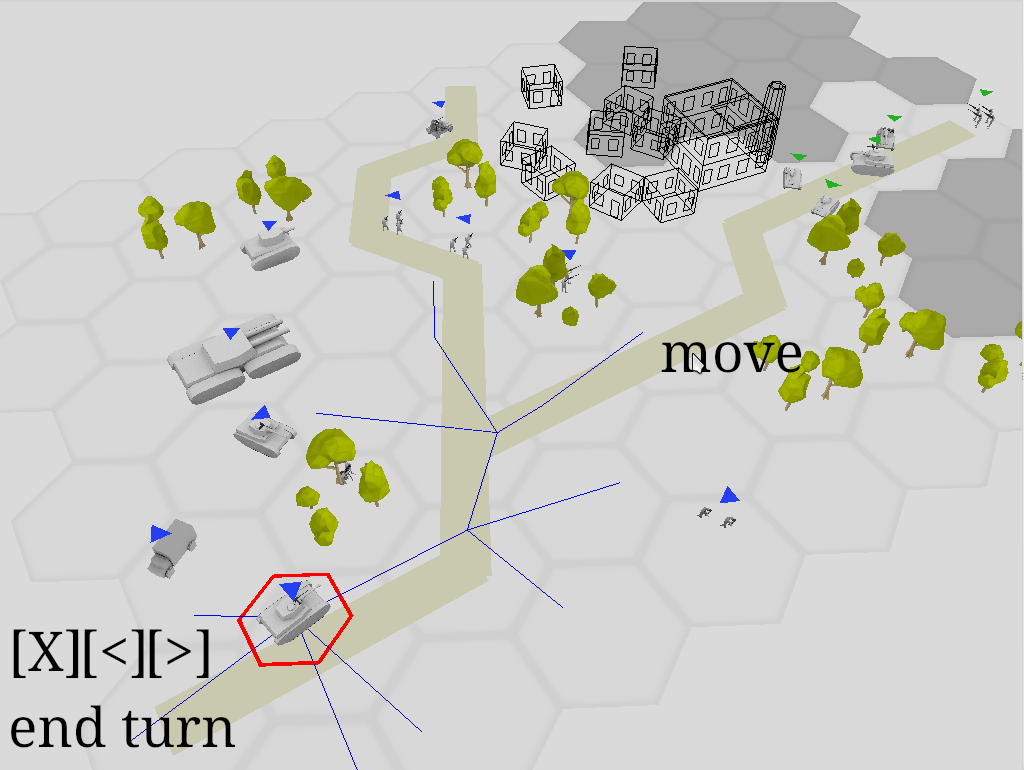
\includegraphics[width=0.9\textwidth]{images/zoc}
\caption{a videogame}
\end{figure}
\end{frame}

\begin{frame}
  \frametitle{So, what can you make with Rust?}
\begin{figure}
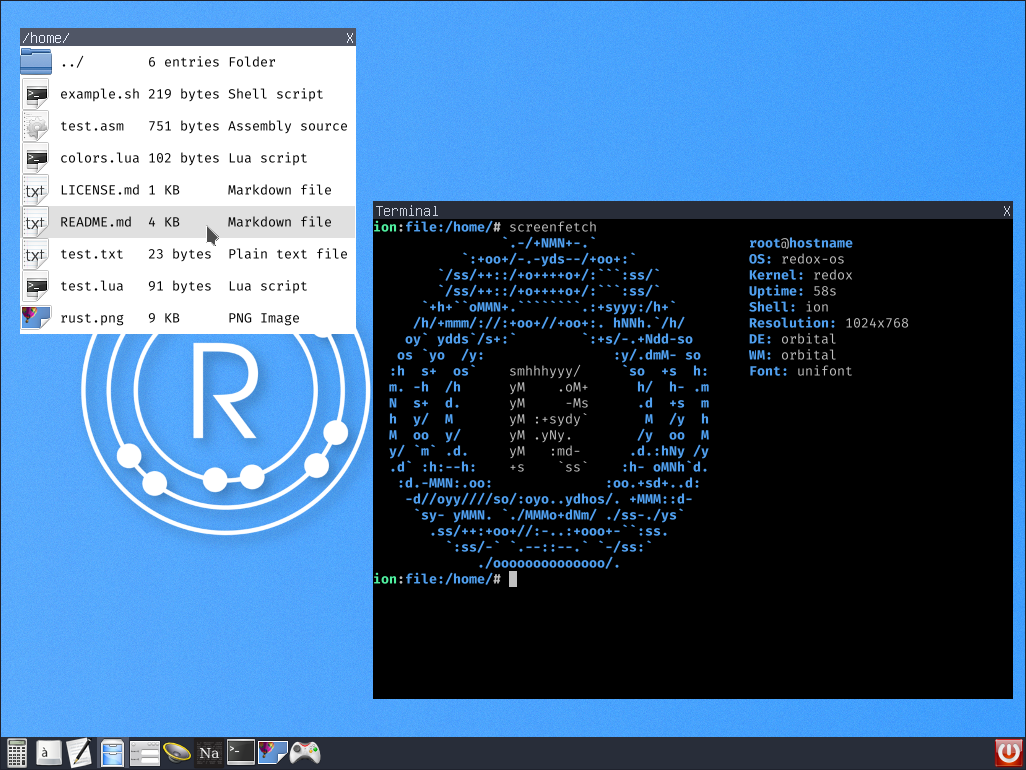
\includegraphics[width=0.9\textwidth]{images/redox}
\caption{an operating system}
\end{figure}
\end{frame}

\begin{frame}
  \frametitle{The catch...}
    \begin{itemize}
      \item{Hard-to-learn...}
      \begin{itemize}
        \item{..because it makes you a better programmer.}
        \item{Incredibly open and friendly community, great tutorials!}
      \end{itemize}
      \item{Young ecosystem}
        \begin{itemize}
          \item{With mature tools}
          \item{Change to really shape the language and ecosystem}
        \end{itemize}
      \item{Longer compile times}
    \end{itemize}
  \end{frame}

  \begin{frame}
    \frametitle{The catch...}
  \begin{figure}
  
\includegraphics[width=0.9\textwidth]{images/compiling}
  \end{figure}
  \end{frame}
% etc
\end{document}
